\documentclass[a4paper,12pt]{article}
\usepackage[utf8]{inputenc}
\usepackage{graphicx}
\usepackage{float}
\usepackage[spanish]{babel}
\usepackage{listings}
\usepackage{xcolor}
\usepackage{courier}
\usepackage[T1]{fontenc}

\definecolor{gris}{RGB}{123, 126, 132}
\definecolor{morado}{RGB}{81, 40, 155}
\definecolor{amarillo}{RGB}{253,151,31}
\definecolor{magenta}{RGB}{249,38,114}

\renewcommand{\lstlistingname}{Archivo}

\lstdefinestyle{customJava}{
    frame=tb,
    language=Java,
    backgroundcolor=\color{white},   
    commentstyle=\itshape\color{gris},
    keywordstyle=\bfseries\color{magenta},
    numberstyle=\color{morado},
    stringstyle=\color{amarillo},
    identifierstyle=\color{black},
    basicstyle=\footnotesize,
    breakatwhitespace=false,         
    breaklines=true,                 
    captionpos=b,
    keepspaces=true,                 
    numbers=left,                    
    numbersep=5pt,                  
    showspaces=false,                
    showstringspaces=false,
    showtabs=false,                  
    tabsize=2,
}

\lstdefinestyle{customXML}{
    frame=tb,
    language=XML,
    backgroundcolor=\color{white},   
    commentstyle=\itshape\color{gris},
    keywordstyle=\bfseries\color{magenta},
    numberstyle=\color{morado},
    stringstyle=\color{amarillo},
    identifierstyle=\color{black},
    basicstyle=\footnotesize,
    breakatwhitespace=false,         
    breaklines=true,                 
    captionpos=b,
    keepspaces=true,                 
    numbers=left,                    
    numbersep=5pt,                  
    showspaces=false,                
    showstringspaces=false,
    showtabs=false,                  
    tabsize=2,
}

%opening
\title{Ejercicio No. 5. Categoria-Producto Hibernate}
\author{Barrera Pérez Carlos Tonatihu \\ Profesor: José Asunción Enríquez 
Zárate \\ Web Application Development \\ Grupo: 3CM9 }

\begin{document}

\maketitle

\newpage
\tableofcontents
\newpage
\section{Introducción}
Este ejercicio tuvo como objetivo desarrollar un proyecto web para el CRUD de 
tiendita que se había trabajado con anterioridad, la base que se 
trabajo fue \ref{fig:bd}.

\begin{figure}[H]
\begin{center}
 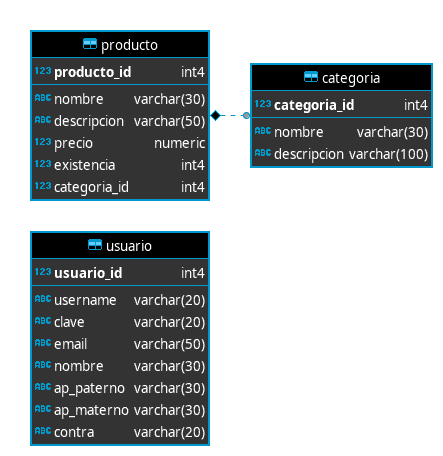
\includegraphics[width=\textwidth]{tiendita.png}
 \caption{Base de datos que se trabajo en PostgreSQL}
 \label{fig:bd}
\end{center}
\end{figure}

También se agrego la funcionalidad de inicio de sesión, generación de reporte, 
de gráficas y envió de estos dos archivos por correo.

\section{Desarrollo}

\begin{lstlisting}[language=Java, style=customJava, 
caption={HibernateUtil.java}, captionpos=b,basicstyle=\fontfamily{cmss}\small]
package me.tonatihu.util;

import org.hibernate.HibernateException;
import org.hibernate.Metamodel;
import org.hibernate.Session;
import org.hibernate.SessionFactory;
import org.hibernate.cfg.Configuration;
import org.hibernate.query.Query;

import javax.persistence.metamodel.EntityType;
import java.util.logging.Level;
import java.util.logging.Logger;

public class HibernateUtil {
    private static final SessionFactory ourSessionFactory;

    static {
        try {
            Configuration configuration = new Configuration();
            configuration.configure();

            ourSessionFactory = configuration.buildSessionFactory();
        } catch (Throwable ex) {
            throw new ExceptionInInitializerError(ex);
        }
    }

    public static Session getSession() throws HibernateException {
        return ourSessionFactory.openSession();
    }
}
\end{lstlisting}

\begin{lstlisting}[language=Java, style=customJava, 
caption={LoginServlet.java}, captionpos=b,basicstyle=\fontfamily{cmss}\small]
package me.tonatihu.controller;

import me.tonatihu.dao.UsuarioDao;
import me.tonatihu.dao.impl.UsuarioDaoImpl;
import me.tonatihu.dto.Usuario;
import me.tonatihu.entity.UsuarioEntity;

import javax.servlet.ServletException;
import javax.servlet.http.HttpServlet;
import javax.servlet.http.HttpServletRequest;
import javax.servlet.http.HttpServletResponse;
import javax.servlet.http.HttpSession;
import java.io.IOException;
import java.util.logging.Level;
import java.util.logging.Logger;

//@WebServlet(name = "LoginServlet")
public class LoginServlet extends HttpServlet {
    private static final Logger LOGGER = 
Logger.getLogger(LoginServlet.class.getName());
    protected void doPost(HttpServletRequest request,
            HttpServletResponse response) throws ServletException, IOException {
        processRequest(request, response);
    }

    protected void doGet(HttpServletRequest request,
            HttpServletResponse response) throws ServletException, IOException {
            processRequest(request, response);
    }

    private void processRequest(HttpServletRequest request, HttpServletResponse 
response)
            throws ServletException, IOException {
        request.setCharacterEncoding("UTF-8");
        String accion = request.getParameter("logout");
        if (accion != null)
            logout(request, response);
        else {
            if (request.getMethod().equals("POST"))
                login(request, response);
            else
                request.getRequestDispatcher("login.jsp").forward(request, 
response);
        }
    }

    private void login(HttpServletRequest request, HttpServletResponse response)
            throws IOException, ServletException {
        UsuarioDao dao = new UsuarioDaoImpl();
        String username = request.getParameter("username");
        String contra = request.getParameter("password");
        UsuarioEntity u = (UsuarioEntity) dao.findByUsernameAndContra(username, 
contra);
        if (u != null) {
            HttpSession session = request.getSession();
            Usuario usuario = new Usuario();
            usuario.setUsername(u.getUsername());
            usuario.setNombreCompleto(u.getNombre() + " " + u.getApPaterno() + " 
" + u.getApMaterno());
            session.setAttribute("USUARIO_SESSION", usuario);
            response.sendRedirect("home");
        } else {
            LOGGER.log(Level.WARNING, "You shall not pass!");
            request.getRequestDispatcher("login.jsp").forward(request, 
response);
        }
    }

    private void logout(HttpServletRequest request, HttpServletResponse 
response)
            throws ServletException, IOException {
        HttpSession session = request.getSession(false);
        session.invalidate();
        request.getRequestDispatcher("login.jsp").forward(request, response);
    }
}
\end{lstlisting}

\begin{lstlisting}[language=Java, style=customJava, 
caption={PerfilServlet.java}, captionpos=b,basicstyle=\fontfamily{cmss}\small]
package me.tonatihu.controller;

import me.tonatihu.dao.impl.UsuarioDaoImpl;
import me.tonatihu.dto.Usuario;
import me.tonatihu.entity.UsuarioEntity;
import me.tonatihu.util.Paginas;

import javax.servlet.ServletException;
import javax.servlet.http.HttpServlet;
import javax.servlet.http.HttpServletRequest;
import javax.servlet.http.HttpServletResponse;
import javax.servlet.http.HttpSession;
import java.io.IOException;

//@WebServlet(name = "PerfilServlet")
public class PerfilServlet extends HttpServlet {
    protected void doPost(HttpServletRequest request,
            HttpServletResponse response) throws ServletException, IOException {
        processRequest(request, response);
    }

    protected void doGet(HttpServletRequest request,
            HttpServletResponse response) throws ServletException, IOException {
        processRequest(request, response);
    }

    private void processRequest(HttpServletRequest request, HttpServletResponse 
response)
            throws ServletException, IOException {
        request.setCharacterEncoding("UTF-8");
        HttpSession session = request.getSession(false);
        Usuario u = (Usuario) session.getAttribute("USUARIO_SESSION");
        UsuarioDaoImpl usuarioDao = new UsuarioDaoImpl();
        UsuarioEntity usuario = usuarioDao.findById(u.getUsername());
        request.setAttribute("usuario", usuario);
        request.setAttribute("PAGINA", Paginas.PERFIL);
        request.getRequestDispatcher("perfil.jsp").forward(request, response);
    }
}
\end{lstlisting}

\begin{lstlisting}[language=Java, style=customJava, 
caption={CategoriasServlet.java}, 
captionpos=b,basicstyle=\fontfamily{cmss}\small]
package me.tonatihu.controller;

import me.tonatihu.entity.CategoriaEntity;
import me.tonatihu.service.CategoriaService;
import me.tonatihu.util.Paginas;

import javax.servlet.ServletException;
import javax.servlet.annotation.WebServlet;
import javax.servlet.http.HttpServlet;
import javax.servlet.http.HttpServletRequest;
import javax.servlet.http.HttpServletResponse;
import java.io.IOException;
import java.util.List;

//@WebServlet(name = "CategoriasServlet")
public class CategoriasServlet extends HttpServlet {
    private void processRequest(HttpServletRequest request,
            HttpServletResponse response) throws ServletException, IOException {
        request.setCharacterEncoding("UTF-8");
        String accion = request.getParameter("accion");
        switch (accion) {
            case "ver":
                listarCategorias(request, response);
                break;
            case "agregar":
                crearCategoria(request, response);
                break;
            case "eliminar":
                eliminarCategoria(request, response);
                break;
            case "guardar":
                almacenarCategoria(request, response);
                break;
            case "editar":
                editarCategoria(request, response);
                break;
        }
    }

    protected void doPost(HttpServletRequest request,
            HttpServletResponse response) throws ServletException, IOException {
        processRequest(request, response);
    }

    protected void doGet(HttpServletRequest request,
            HttpServletResponse response) throws ServletException, IOException {
        processRequest(request, response);
    }

    private void editarCategoria(HttpServletRequest request,
            HttpServletResponse response) throws ServletException, IOException {
        CategoriaService service = new CategoriaService();
        CategoriaEntity c = 
service.findById(Integer.parseInt(request.getParameter("id")));
        request.setAttribute("categoria", c);
        request.setAttribute("PAGINA", Paginas.VER_CATEGORIAS);
        request.getRequestDispatcher("formCategoria.jsp").forward(request, 
response);
    }

    private void listarCategorias(HttpServletRequest request, 
HttpServletResponse response)
            throws ServletException, IOException {
        CategoriaService categoriaService = new CategoriaService();
        List<CategoriaEntity> lista = categoriaService.findAll();
        request.setAttribute("categorias", lista);
        request.setAttribute("PAGINA", Paginas.VER_CATEGORIAS);
        request.getRequestDispatcher("listaCategorias.jsp").forward(request, 
response);
    }

    private void crearCategoria(HttpServletRequest request,
            HttpServletResponse response) throws ServletException, IOException {
        request.setAttribute("PAGINA", Paginas.AGREGAR_CATEGORIA);
        request.getRequestDispatcher("formCategoria.jsp").forward(request, 
response);
    }

    private void eliminarCategoria(HttpServletRequest request, 
HttpServletResponse response)
            throws IOException {
        CategoriaService categoriaService = new CategoriaService();
        int id = Integer.parseInt(request.getParameter("id"));
        categoriaService.delete(id);
        response.sendRedirect("categorias?accion=ver");
    }

    private void almacenarCategoria(HttpServletRequest request, 
HttpServletResponse response)
            throws IOException {
        CategoriaEntity c = new CategoriaEntity();
        CategoriaService service = new CategoriaService();
        if (request.getParameter("id") == null || 
request.getParameter("id").isEmpty()) {
            c.setNombre(request.getParameter("nombre"));
            c.setDescripcion(request.getParameter("descripcion"));
            service.create(c);
        } else {
            c.setCategoriaId(Integer.parseInt(request.getParameter("id")));
            c.setNombre(request.getParameter("nombre"));
            c.setDescripcion(request.getParameter("descripcion"));
            service.update(c);
        }
        response.sendRedirect("categorias?accion=ver");
    }
}
\end{lstlisting}

\begin{lstlisting}[language=Java, style=customJava, 
caption={ProductosServlet.java}, 
captionpos=b,basicstyle=\fontfamily{cmss}\small]
package me.tonatihu.controller;

import me.tonatihu.dao.impl.ProductoDaoImpl;
import me.tonatihu.entity.CategoriaEntity;
import me.tonatihu.entity.ProductoEntity;
import me.tonatihu.service.CategoriaService;
import me.tonatihu.util.Paginas;

import javax.servlet.ServletException;
import javax.servlet.http.HttpServlet;
import javax.servlet.http.HttpServletRequest;
import javax.servlet.http.HttpServletResponse;
import java.io.IOException;
import java.math.BigDecimal;
import java.util.List;

//@WebServlet(name = "ProductosServlet")
public class ProductosServlet extends HttpServlet {
    protected void doPost(HttpServletRequest request,
            HttpServletResponse response) throws ServletException, IOException {
        processRequest(request, response);
    }

    protected void doGet(HttpServletRequest request,
            HttpServletResponse response) throws ServletException, IOException {
        processRequest(request, response);
    }

    private void processRequest(HttpServletRequest request, HttpServletResponse 
response)
            throws ServletException, IOException {
        request.setCharacterEncoding("UTF-8");
        String accion = request.getParameter("accion");
        switch (accion) {
            case "ver":
                listar(request, response);
                break;
            case "agregar":
                crear(request, response);
                break;
            case "eliminar":
                eliminar(request, response);
                break;
            case "guardar":
                guardar(request, response);
                break;
            case "editar":
                editar(request, response);
                break;
        }
    }

    private void crear(HttpServletRequest request, HttpServletResponse response) 
throws ServletException, IOException {
        CategoriaService service = new CategoriaService();
        request.setAttribute("PAGINA", Paginas.AGREGAR_PRODUCTO);
        request.setAttribute("categorias", service.findAll());
        request.getRequestDispatcher("formProducto.jsp").forward(request, 
response);
    }

    private void guardar(HttpServletRequest request, HttpServletResponse 
response)
            throws IOException {
        ProductoEntity producto = new ProductoEntity();
        ProductoDaoImpl productoDao = new ProductoDaoImpl();
        CategoriaEntity c = new CategoriaEntity();

        c.setCategoriaId(Integer.parseInt(request.getParameter("categoria")));

        producto.setNombre(request.getParameter("nombre"));
        producto.setDescripcion(request.getParameter("descripcion"));
        
producto.setExistencia(Integer.parseInt(request.getParameter("existencia")));
        
producto.setPrecio(BigDecimal.valueOf(Double.valueOf(request.getParameter("preci
o"))));
        producto.setCategoria(c);
        if (request.getParameter("id") == null || 
request.getParameter("id").isEmpty()) {
            productoDao.create(producto);
        } else {
            
producto.setProductoId(Integer.parseInt(request.getParameter("id")));
            productoDao.update(producto);
        }
        response.sendRedirect("productos?accion=ver");
    }

    private void eliminar(HttpServletRequest request, HttpServletResponse 
response)
            throws IOException {
        ProductoDaoImpl dao = new ProductoDaoImpl();
        int id = Integer.parseInt(request.getParameter("id"));
        ProductoEntity p = dao.findById(id);
        dao.delete(p);
        response.sendRedirect("productos?accion=ver");
    }

    private void editar(HttpServletRequest request, HttpServletResponse 
response)
            throws ServletException, IOException {
        ProductoDaoImpl dao = new ProductoDaoImpl();
        CategoriaService service = new CategoriaService();
        ProductoEntity p= 
dao.findById(Integer.parseInt(request.getParameter("id")));
        request.setAttribute("producto", p);
        request.setAttribute("categorias", service.findAll());
        request.setAttribute("PAGINA", Paginas.VER_PRODUCTOS);
        request.getRequestDispatcher("formProducto.jsp").forward(request, 
response);
    }

    private void listar(HttpServletRequest request, HttpServletResponse 
response)
            throws ServletException, IOException {
        request.setAttribute("PAGINA", Paginas.VER_PRODUCTOS);
        ProductoDaoImpl dao = new ProductoDaoImpl();
        List<ProductoEntity> lista = ((ProductoDaoImpl) dao).findAll();
        request.setAttribute("productos", lista);
        request.getRequestDispatcher("listaProductos.jsp").forward(request, 
response);
    }

}
\end{lstlisting}

\begin{lstlisting}[language=Java, style=customJava, 
caption={GenericDao.java}, captionpos=b,basicstyle=\fontfamily{cmss}\small]
package me.tonatihu.dao;

import me.tonatihu.util.HibernateUtil;
import org.hibernate.Session;
import org.hibernate.Transaction;

import java.io.Serializable;
import java.util.List;

/**
 * @author tonatihu
 * Created on 3/17/19
 */

public abstract class GenericDao <T, Id extends Serializable>{
    private Session currentSession;
    private Transaction currentTransaction;

    public void openCurrentSession() {
        currentSession = HibernateUtil.getSession();
    }

    public void openCurrentSessionWithTransaction() {
        currentSession = HibernateUtil.getSession();
        currentTransaction = currentSession.beginTransaction();
    }

    public void closeCurrentSession() {
        currentSession.close();
    }

    public void closeCurrentSessionwithTransaction() {
        currentTransaction.commit();
        currentSession.close();
    }

    public void rollback() {
        if (currentTransaction != null)
            currentTransaction.rollback();
    }

    protected Session getCurrentSession() {
        return currentSession;
    }

    public abstract void create(T entity);
    public abstract void update(T entity);
    public abstract T findById(Id id);
    public abstract void delete(T entity);
    public abstract List<T> findAll();
}
\end{lstlisting}

\begin{lstlisting}[language=Java, style=customJava, 
caption={UsuarioDao.java}, captionpos=b,basicstyle=\fontfamily{cmss}\small]
package me.tonatihu.dao;

import java.io.Serializable;

/**
 * @author tonatihu
 * Created on 3/17/19
 */

public interface UsuarioDao<T, Id extends Serializable> {
    T findByUsernameAndContra(String username, String contra);
    T findByUsername(String username);
}
\end{lstlisting}

\begin{lstlisting}[language=Java, style=customJava, 
caption={UsuarioDaoImpl.java}, captionpos=b,basicstyle=\fontfamily{cmss}\small]
package me.tonatihu.dao.impl;

import me.tonatihu.dao.GenericDao;
import me.tonatihu.dao.UsuarioDao;
import me.tonatihu.entity.UsuarioEntity;
import org.hibernate.query.Query;

import java.util.List;

/**
 * @author tonatihu
 * Created on 3/17/19
 */

public class UsuarioDaoImpl extends GenericDao<UsuarioEntity, String> implements 
UsuarioDao<UsuarioEntity, String> {
    private static final String FIND_BY_USERNAME_AND_CONTRA = "from 
UsuarioEntity where username=:u and contra=:p";
    private static final String FIND_BY_USERNAME = "from UsuarioEntity where 
username=:u";

    @Override
    public UsuarioEntity findByUsernameAndContra(String username, String contra) 
{
        openCurrentSession();
        Query query = 
getCurrentSession().createQuery(FIND_BY_USERNAME_AND_CONTRA);
        query.setParameter("u", username);
        query.setParameter("p", contra);
        UsuarioEntity usuario = (UsuarioEntity) query.uniqueResult();
        closeCurrentSession();
        return usuario;
    }

    @Override
    public UsuarioEntity findByUsername(String username) {
        openCurrentSession();
        Query query = getCurrentSession().createQuery(FIND_BY_USERNAME);
        query.setParameter("u", username);
        UsuarioEntity usuario = (UsuarioEntity) query.uniqueResult();
        closeCurrentSession();
        return usuario;
    }

    @Override
    public void create(UsuarioEntity entity) {

    }

    @Override
    public void update(UsuarioEntity entity) {

    }

    @Override
    public UsuarioEntity findById(String s) {
        openCurrentSession();
        UsuarioEntity usuario = getCurrentSession().get(UsuarioEntity.class, s);
        closeCurrentSession();
        return usuario;
    }

    @Override
    public void delete(UsuarioEntity entity) {

    }

    @Override
    public List<UsuarioEntity> findAll() {
        return null;
    }
}
\end{lstlisting}

\begin{lstlisting}[language=Java, style=customJava, 
caption={CategoriaDaoImpl.java}, 
captionpos=b,basicstyle=\fontfamily{cmss}\small]
package me.tonatihu.dao.impl;

import me.tonatihu.dao.GenericDao;
import me.tonatihu.entity.CategoriaEntity;

import java.util.List;

/**
 * @author tonatihu
 * Created on 3/11/19
 */

public class CategoriaDaoImpl extends GenericDao<CategoriaEntity, Integer> {
    @Override
    public void create(CategoriaEntity entity) {
        getCurrentSession().persist(entity);
    }

    @Override
    public void update(CategoriaEntity entity) {
        getCurrentSession().update(entity);
    }

    @Override
    public CategoriaEntity findById(Integer id) {
        return getCurrentSession().get(CategoriaEntity.class, id);
    }

    @Override
    public void delete(CategoriaEntity entity) {
        getCurrentSession().delete(entity);
    }

    @Override
    @SuppressWarnings("unchecked")
    public List<CategoriaEntity> findAll() {
        return (List<CategoriaEntity>) getCurrentSession().createQuery("from 
CategoriaEntity ").list();
    }
}
\end{lstlisting}

\begin{lstlisting}[language=Java, style=customJava, 
caption={ProductoDaoImpl.java}, captionpos=b,basicstyle=\fontfamily{cmss}\small]
package me.tonatihu.dao.impl;

import me.tonatihu.dao.GenericDao;
import me.tonatihu.dto.Dato;
import me.tonatihu.entity.ProductoEntity;
import org.hibernate.HibernateException;

import java.util.ArrayList;
import java.util.List;
import java.util.logging.Level;
import java.util.logging.Logger;


/**
 * @author tonatihu
 * Created on 3/11/19
 */

public class ProductoDaoImpl extends GenericDao<ProductoEntity, Integer> {
    private static final Logger LOGGER = 
Logger.getLogger(ProductoDaoImpl.class.getName());
    @Override
    public void create(ProductoEntity entity) {
        openCurrentSessionWithTransaction();
        try {
            getCurrentSession().save(entity);
        } catch (HibernateException hehe) {
            LOGGER.log(Level.SEVERE, "Error en create", hehe);
            rollback();
        } finally {
            closeCurrentSessionwithTransaction();
        }
    }

    @Override
    public void update(ProductoEntity entity) {
        openCurrentSessionWithTransaction();
        try {
            getCurrentSession().update(entity);
        } catch (HibernateException hehe) {
            LOGGER.log(Level.SEVERE, "Error en update", hehe);
            rollback();
        } finally {
            closeCurrentSessionwithTransaction();
        }
    }

    @Override
    public ProductoEntity findById(Integer integer) {
        openCurrentSession();
        ProductoEntity productoEntity = 
getCurrentSession().get(ProductoEntity.class, integer);
        closeCurrentSession();
        return productoEntity;
    }

    @Override
    public void delete(ProductoEntity entity) {
        openCurrentSessionWithTransaction();
        try {
            getCurrentSession().delete(entity);
        } catch (HibernateException hehe) {
            LOGGER.log(Level.SEVERE, "Error en delete", hehe);
            rollback();
        } finally {
            closeCurrentSessionwithTransaction();
        }
    }

    @Override
    @SuppressWarnings("unchecked")
    public List<ProductoEntity> findAll() {
        openCurrentSession();
        List<ProductoEntity> lista = (List<ProductoEntity>) getCurrentSession()
                .createQuery("from ProductoEntity").list();
        closeCurrentSession();
        return lista;
    }

    public List<Dato> getDatos() {
        openCurrentSession();
        List lista = getCurrentSession()
                .createQuery("select c.nombre as nombre, count(p.nombre) as 
catidad " +
                        "from CategoriaEntity as c left join c.productos as p " 
+
                        "group by c.nombre").getResultList();
        List<Dato> datos = new ArrayList<>();
        for (Object o : lista) {
            Object[] filas = (Object[]) o;
            datos.add(new Dato((String) filas[0], ((Long)filas[1]).intValue()));
        }
        closeCurrentSession();
        return datos;
    }
    private static void printResult(Object result) {
        if (result == null) {
            System.out.print("NULL");
        } else if (result instanceof Object[]) {
            Object[] row = (Object[]) result;
            System.out.print("[");
            for (Object o : row) {
                printResult(o);
            }
            System.out.print("]");
        } else if (result instanceof Long || result instanceof Double
                || result instanceof String) {
            System.out.print("Chido: " + result.getClass().getName() + ": " + 
result);
        } else {
            System.out.print("Resultado: " + result);
        }
    }

}
\end{lstlisting}

\section{Pruebas}

\begin{figure}[H]
\begin{center}
 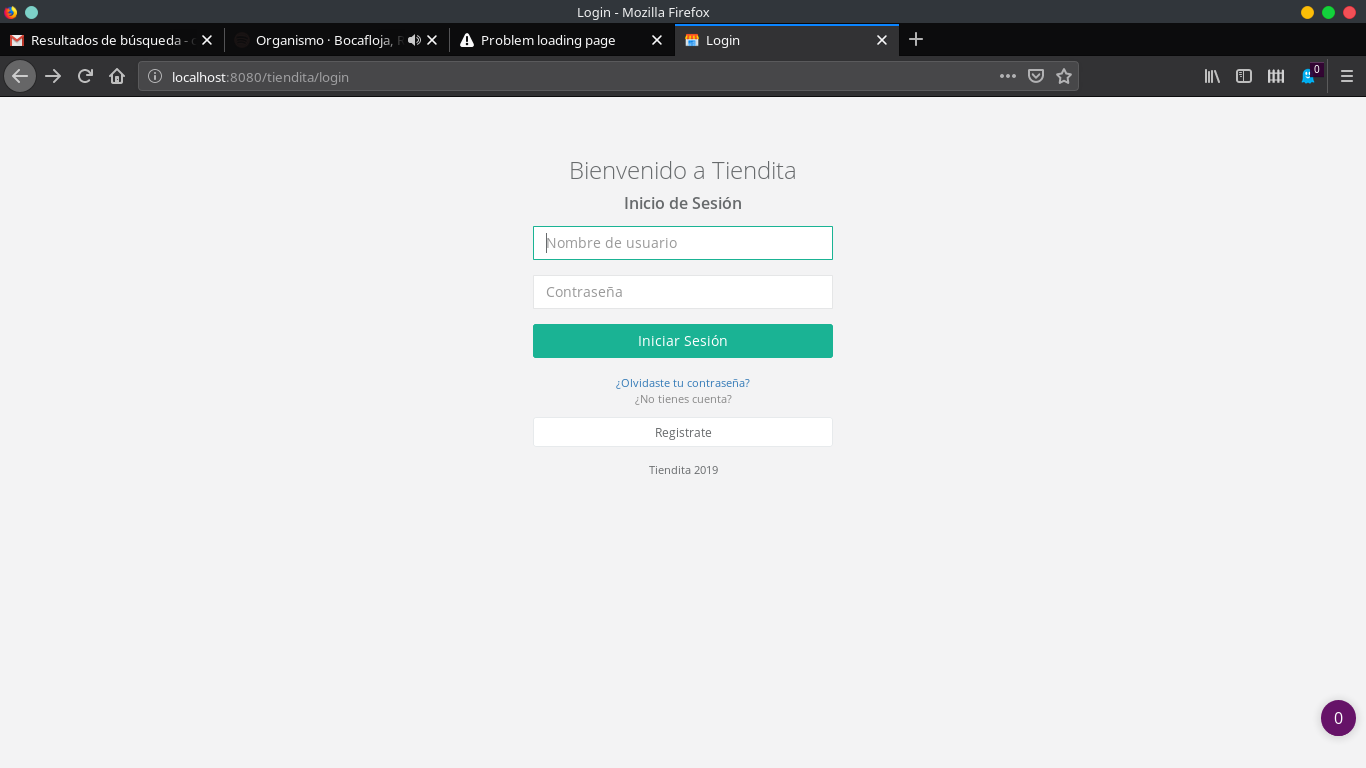
\includegraphics[width=\textwidth]{login.png}
 \caption{Login}
 \label{fig:login}
\end{center}
\end{figure}

\begin{figure}[H]
\begin{center}
 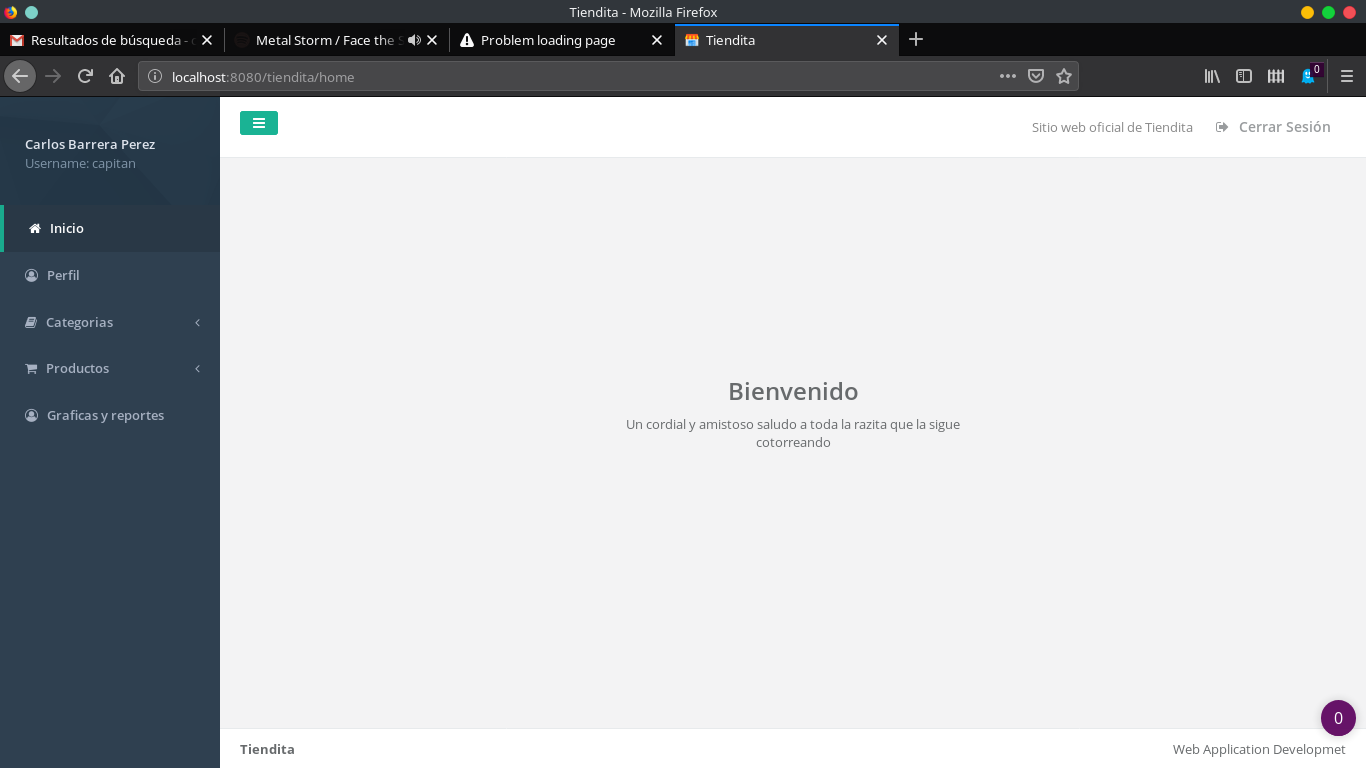
\includegraphics[width=\textwidth]{home.png}
 \caption{Home}
 \label{fig:home}
\end{center}
\end{figure}

\begin{figure}[H]
\begin{center}
 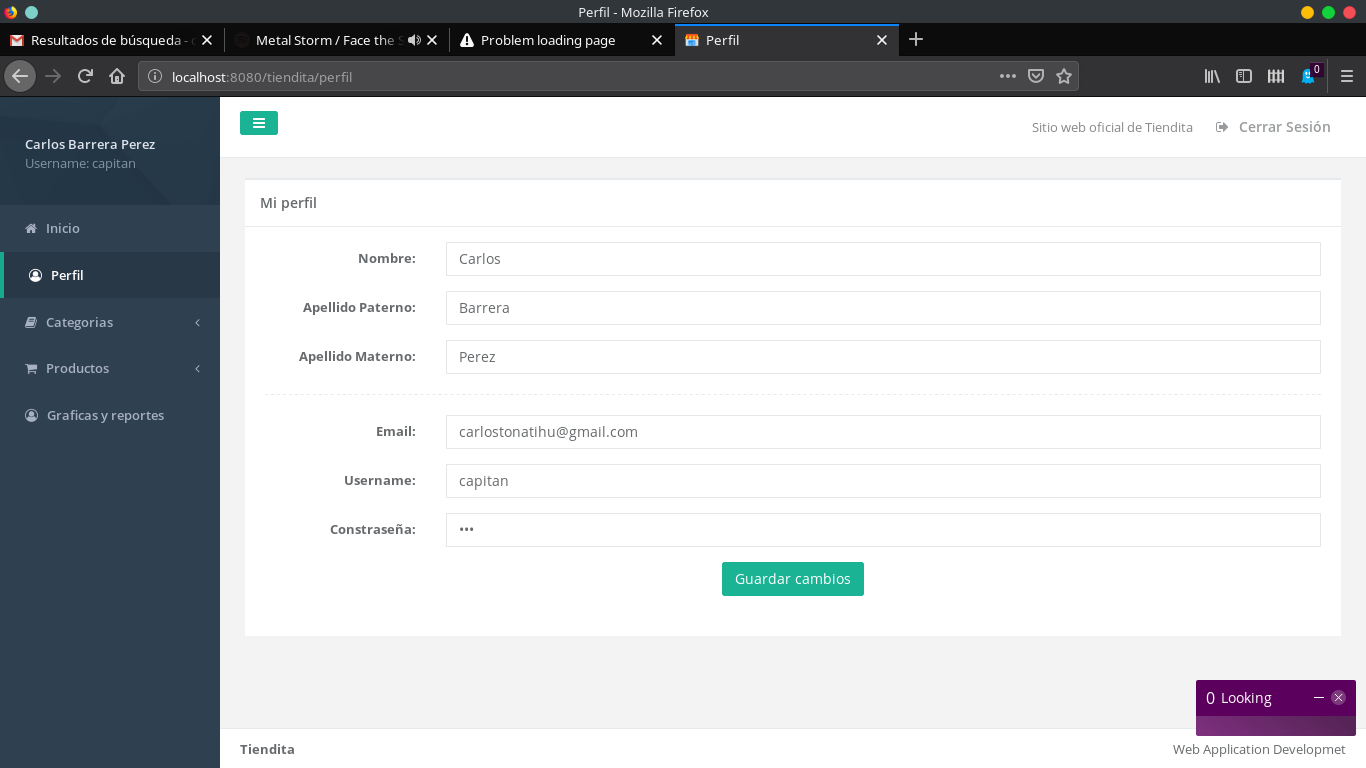
\includegraphics[width=\textwidth]{perfil.png}
 \caption{Perfil}
 \label{fig:perfil}
\end{center}
\end{figure}

\begin{figure}[H]
\begin{center}
 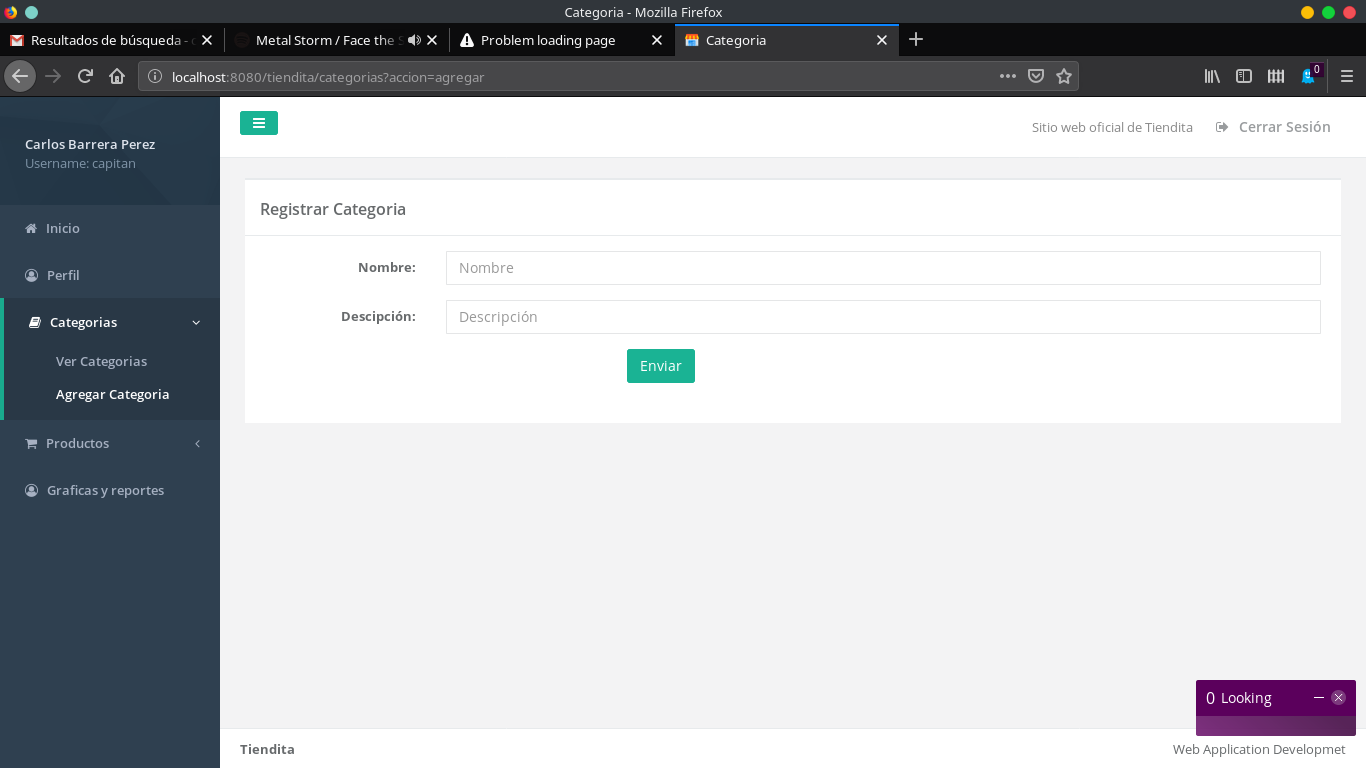
\includegraphics[width=\textwidth]{agregar_categoria.png}
 \caption{Agregar categoría}
 \label{fig:agregar_categoria}
\end{center}
\end{figure}

\begin{figure}[H]
\begin{center}
 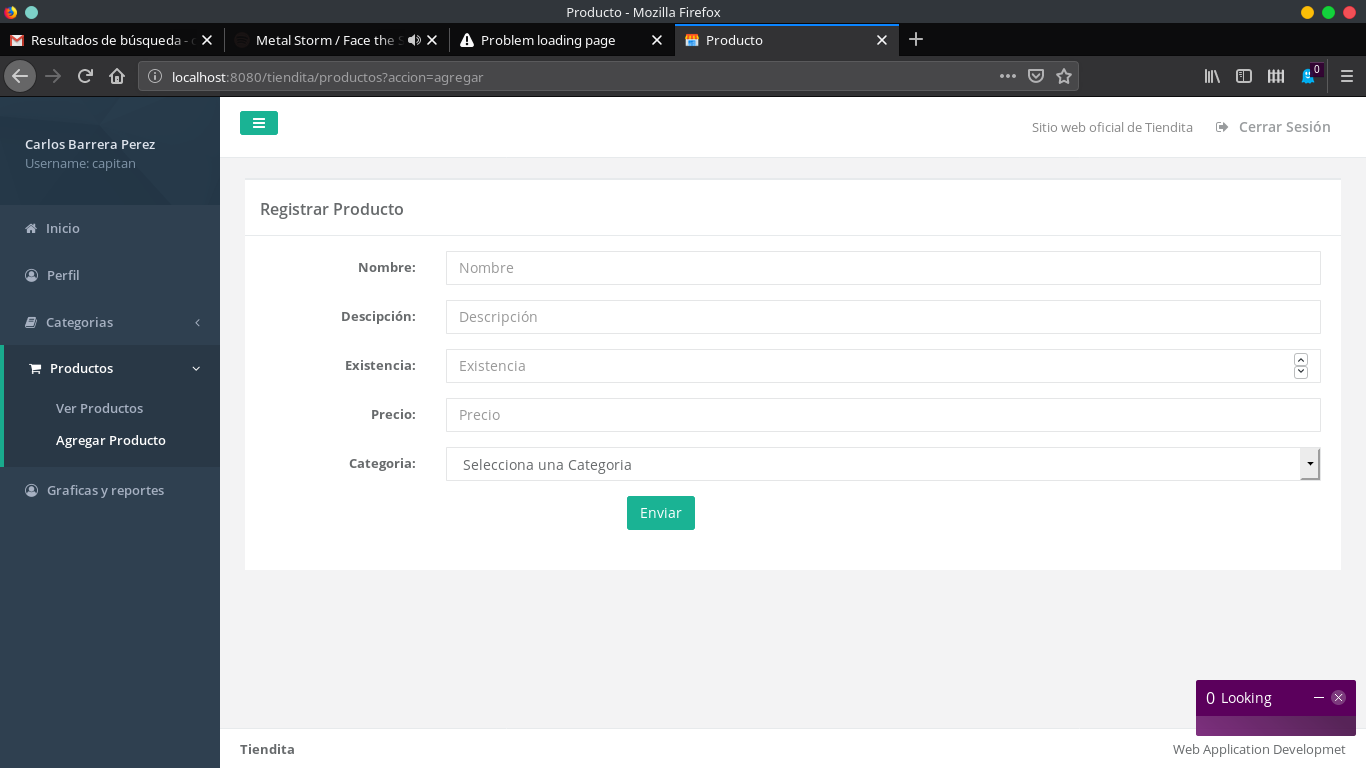
\includegraphics[width=\textwidth]{agregar_producto.png}
 \caption{Agregar producto}
 \label{fig:agregar_producto}
\end{center}
\end{figure}

\begin{figure}[H]
\begin{center}
 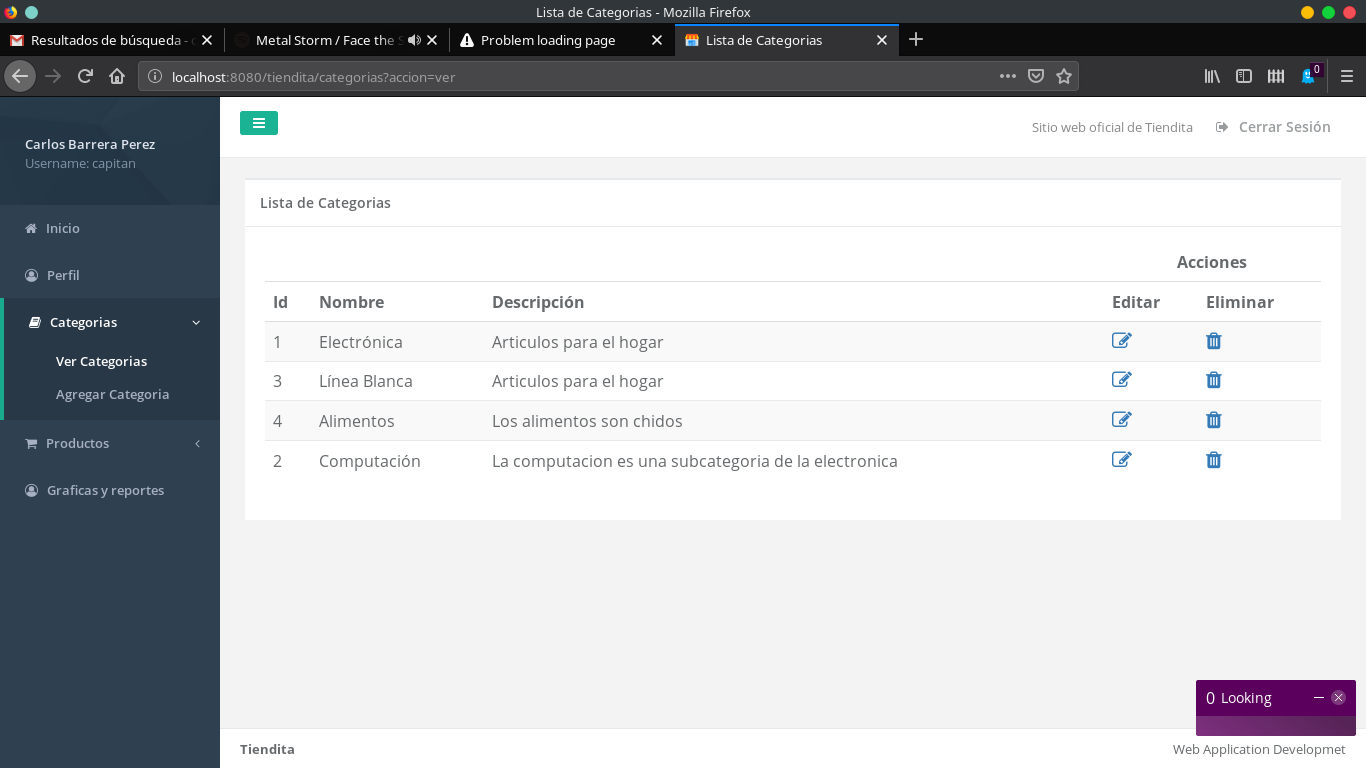
\includegraphics[width=\textwidth]{ver_categorias.png}
 \caption{Ver categorías}
 \label{fig:ver_categorias}
\end{center}
\end{figure}

\begin{figure}[H]
\begin{center}
 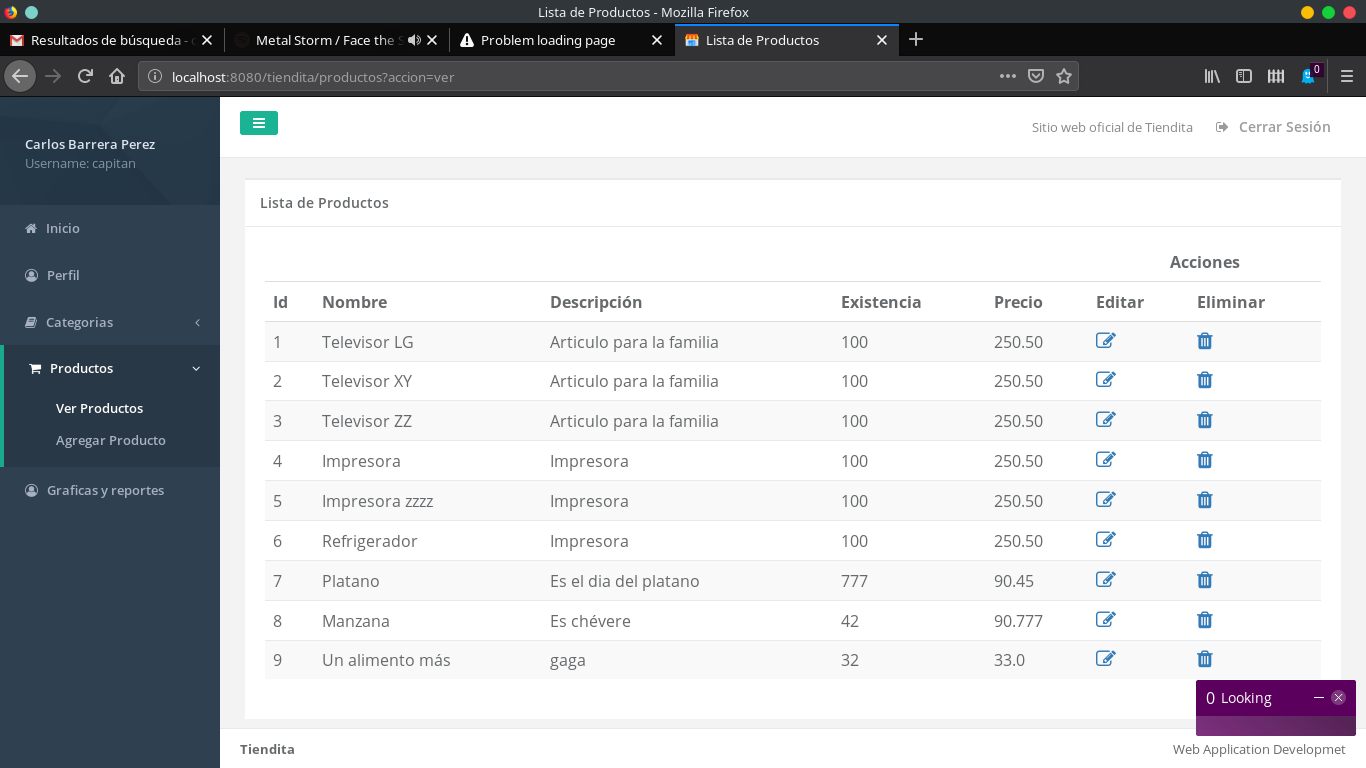
\includegraphics[width=\textwidth]{ver_productos.png}
 \caption{Ver productos}
 \label{fig:ver_productos}
\end{center}
\end{figure}

\begin{figure}[H]
\begin{center}
 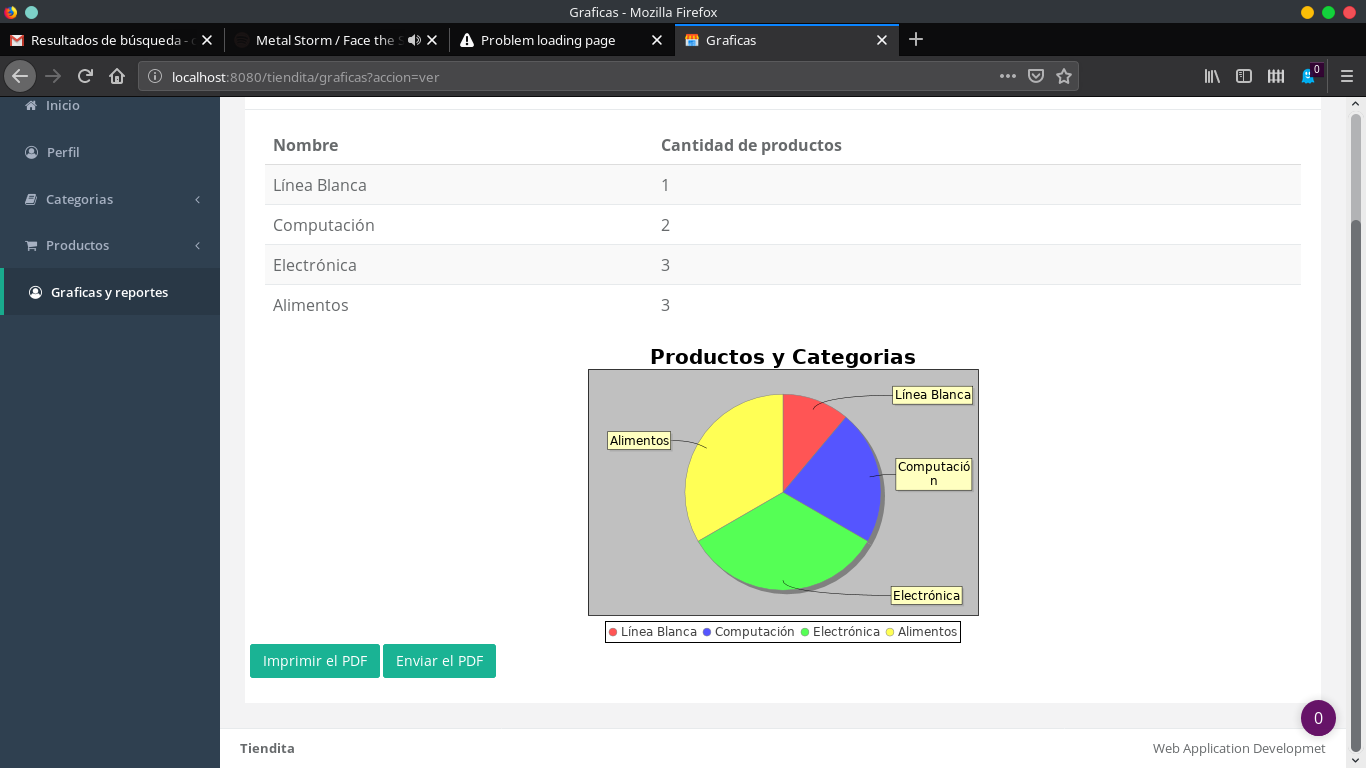
\includegraphics[width=\textwidth]{graficas.png}
 \caption{Gráficas}
 \label{fig:graficas}
\end{center}
\end{figure}

\begin{figure}[H]
\begin{center}
 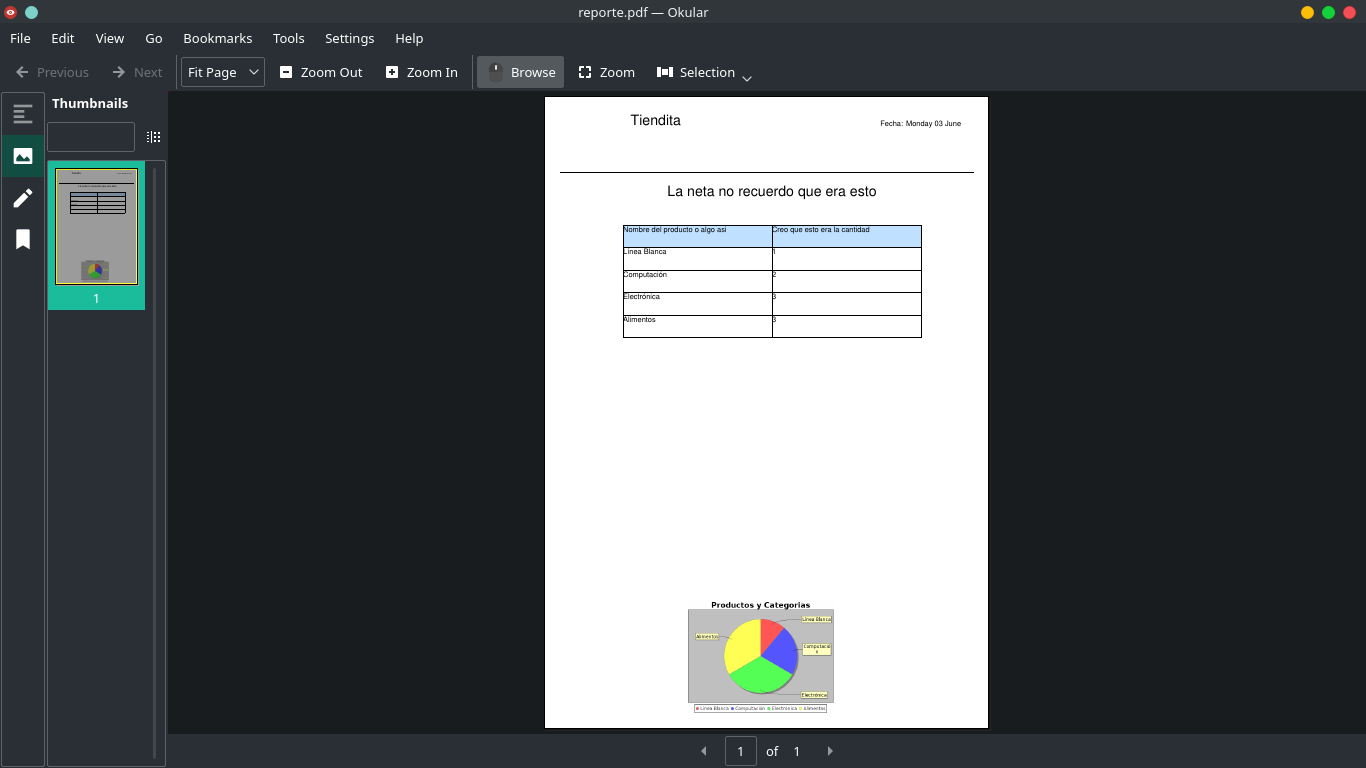
\includegraphics[width=\textwidth]{reporte.png}
 \caption{Reporte}
 \label{fig:reporte}
\end{center}
\end{figure}

\begin{figure}[H]
\begin{center}
 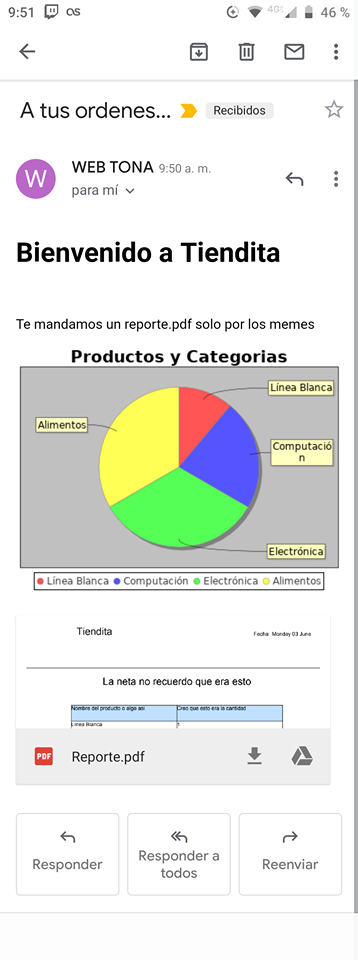
\includegraphics[width=8cm]{celular.png}
 \caption{Envío del reporte y la gráfica por email}
 \label{fig:celular}
\end{center}
\end{figure}

\section{Conclusiones}
La parte complicada de esta materia fue el generar el reporte debido a que 
trabajar con jasper no es tan sencillo como parece, por lo cual consumió gran 
parte de la elaboración de esta practica, el resto no fue tan difícil debido a 
que ya se había trabajado con cosas similares en ejercicios anteriores

\end{document}
